% !TEX program = lualatex
%%%%%%%%%%%%%%%%%%%%%%%%%%%%%%%%%%%%%%%%%%%%%%%%%%%%%%%%%%%%%%
%% Presentation template and short Beamer example/tutorial.
%% Vincent Labatut 2017-19 <vincent.labatut@univ-avignon.fr>
%%%%%%%%%%%%%%%%%%%%%%%%%%%%%%%%%%%%%%%%%%%%%%%%%%%%%%%%%%%%%%
% setup beamer
\documentclass[10pt,    % default is 11pt, use 10pt for more compact slides
%    handout,            % collapse all overlays (=animations) and video-invert console text
    english,            % presentation language (theme supports only french & english)
    xcolor=table,       % colors in the tables
    envcountsect,        % include section number in theorem numbers
    aspectratio=1610
]{beamer}
\usepackage{gensymb}
\usepackage[absolute,overlay]{textpos}

%%%%%%%%%%%%%%%%%%%%%%%%%%%%%%%%%%%%%%%%%%%%%%%%%%%%%%%%%%%%%%
% setup the theme
%\usepackage{./sty/beamerthemeAU}         % no option at all
\usepackage[light]{./sty/beamerthemeAU}   % the "light" option only changes the title and section pages

%%%%%%%%%%%%%%%%%%%%%%%%%%%%%%%%%%%%%%%%%%%%%%%%%%%%%%%%%%%%%%
% setup side notes
\usepackage{pgfpages}                                   % comment all 3 below lines to hide notes
%\setbeameroption{show notes}                           % alternate content and note slides
%\setbeameroption{show only notes}                      % only note slides
%\setbeameroption{show notes on second screen=right}    % dualscreen: right, left, top, bottom

\usepackage{tikz}
%\usetikzlibrary{shapes.geometric, arrows}
\usetikzlibrary{arrows,shapes,positioning,shadows,trees}
\tikzset{
  basic/.style  = {draw, text width=5cm, drop shadow, font=\sffamily, rectangle},
  root/.style   = {basic, rounded corners=2pt, thin, align=center,
                   fill=cyan!50},
  level 2/.style = {basic, rounded corners=2pt, thin,align=center, fill=cyan!20,
                   text width=10em},
  level 3/.style = {basic, rounded corners=2pt, thin, align=left, fill=green!15, 
                   text width=8em}
}


%%%%%%%%%%%%%%%%%%%%%%%%%%%%%%%%%%%%%%%%%%%%%%%%%%%%%%%%%%%%%%
% name of the biblatex file
%\addbibresource{biblio.bib}
\setbeamertemplate{footline}[frame number]


%%%%%%%%%%%%%%%%%%%%%%%%%%%%%%%%%%%%%%%%%%%%%%%%%%%%%%%%%%%%%%
% title and subtitle of the presentation (the latter is optional)
\title[] % leave empty for no title in footer
{Electrical Impedance Tomography for Perfusion Imaging and Monitoring}
\subtitle{Thesis Defence Presentation}
%%%%%%%%%%%%%%%%%%%%%%%%%%%%%%%%%%%%%%%%%%%%%%%%%%%%%%%%%%%%%%
% date of the presentation (leave empty for no date, default is today)
\date[] % leave empty for no date in footer
    {\today}
%%%%%%%%%%%%%%%%%%%%%%%%%%%%%%%%%%%%%%%%%%%%%%%%%%%%%%%%%%%%%%
% authors and their affiliations (the latter is optional)
\author[] % leave empty for no author in footer
{Symon~Stowe} % \alert{Author~Two}} %\inst{} \and \underline{FirstnameB~LastnameB}\inst{2} \and FirstnameC~LastnameC\textsuperscript{1,2}}
\institute[] % (short affiliation not used in this theme)
{\texttt{symonstowe@sce.carleton.ca}
}

%%%%%%%%%%%%%%%%%%%%%%%%%%%%%%%%%%%%%%%%%%%%%%%%%%%%%%%%%%%%%%
% optional: additional logo (ex. lab)
\titlegraphic{
\includegraphics[width=3.5cm]{carleton-university-logo.pdf}\hspace{5cm}}
% if you want several logos, put them in a box
%\titlegraphic{\parbox{3cm}{\includegraphics[width=3cm,]{images/ceri_logo.pdf}\newline\includegraphics[width=3cm,]{images/lia_logo.pdf}}}
%%%%%%%%%%%%%%%%%%%%%%%%%%%%%%%%%%%%%%%%%%%%%%%%%%%%%%%%%%%%%%
\graphicspath{{imgs/}}	% Root directory of the pictures 
%%%%%%%%%%%%%%%%%%%%%%%%%%%%%%%%%%%%%%%%%%%%%%%%%%%%%%%%%%%%%%
\begin{document}
%%% title page
	
\begin{frame}
  \titlepage
\end{frame}

\begin{frame}
	\frametitle{Overview}
	\begin{enumerate}
		\item Thesis Goals
		\item Contributions
		\item Background
		\item Methods and Results
		\item Conclusions
		\item Future Work 
	\end{enumerate}
\end{frame}

\begin{frame}
	\frametitle{Thesis Goals}
	\begin{figure}
		\centering
	%\begin{tikzpicture}
	%<code goes here>
	%\end{tikzpicture}
	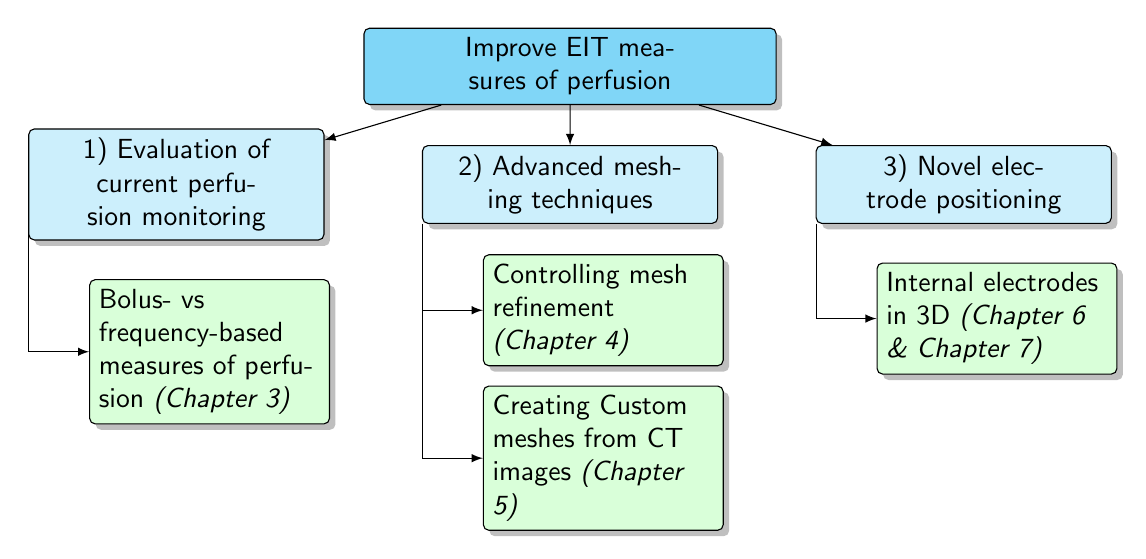
\begin{tikzpicture}[
	  level 1/.style={sibling distance=50mm},
	  edge from parent/.style={->,draw},
	  >=latex]
	
	% root of the the initial tree, level 1
	\node[root] {Improve EIT measures of perfusion}
	% The first level, as children of the initial tree
	  child {node[level 2] (c1) {1) Evaluation of current perfusion monitoring}}
	  child {node[level 2] (c2) {2) Advanced meshing techniques}}
	  child {node[level 2] (c3) {3) Novel electrode positioning}};
	
	% The second level, relatively positioned nodes
	\begin{scope}[every node/.style={level 3}]
	\node [below of = c1, xshift=12pt, yshift=-32pt] (c11) {Bolus- vs 
	frequency-based measures of perfusion \emph{(Chapter 3)}}; 
	
	\node [below of = c2, xshift=12pt, yshift=-17pt] (c21) 
	{Controlling mesh refinement\\ \emph{(Chapter 4)}};
	\node [below of = c21, yshift=-25pt] (c22) 
	{Creating Custom meshes from CT images \emph{(Chapter 5)}};
	\node [below of = c3, xshift=12pt, yshift=-20pt] (c31) 
	{Internal electrodes in 3D \emph{(Chapter 6 \& Chapter 7)}};
	\end{scope}
	
	% lines from each level 1 node to every one of its "children"
	\foreach \value in {1}
	  \draw[->] (c1.195) |- (c1\value.west);
	
	\foreach \value in {1,2}
	  \draw[->] (c2.195) |- (c2\value.west);
	
	\foreach \value in {1}
	  \draw[->] (c3.195) |- (c3\value.west);
	
	\end{tikzpicture}
\end{figure}
\end{frame}

\begin{frame}
	\frametitle{Contributions}    
	\begin{columns}[c]
		\begin{column}{0.5\textwidth}
			\begin{enumerate}
				\item A mesh analysis technique to reduce error in sensitivity calculations on 
				cylindrical meshes (\alert{Chapter 4}). \\ \vspace{4mm}
				\item A tool to generate custom meshes of exterior and lung boundaries from CT iamges
				(\alert{Chapter 5}).
			\end{enumerate}
		\end{column}
		\begin{column}{0.5\textwidth}
			\begin{enumerate}
				\setcounter{enumi}{2}
				\item An analysis of 3D electrode placements with internal electrodes on internal 
				sensitivity (\alert{Chapter 6}). \\ \vspace{4mm}
				\item A method to reconstruct images using internal electrode measurements in the
				presence of movement (\alert{Chapter 7}).
			\end{enumerate}
		\end{column}
	\end{columns}
\end{frame}

\begin{frame}
	\frametitle{Background: EIT}
	\begin{figure}
		\centering
	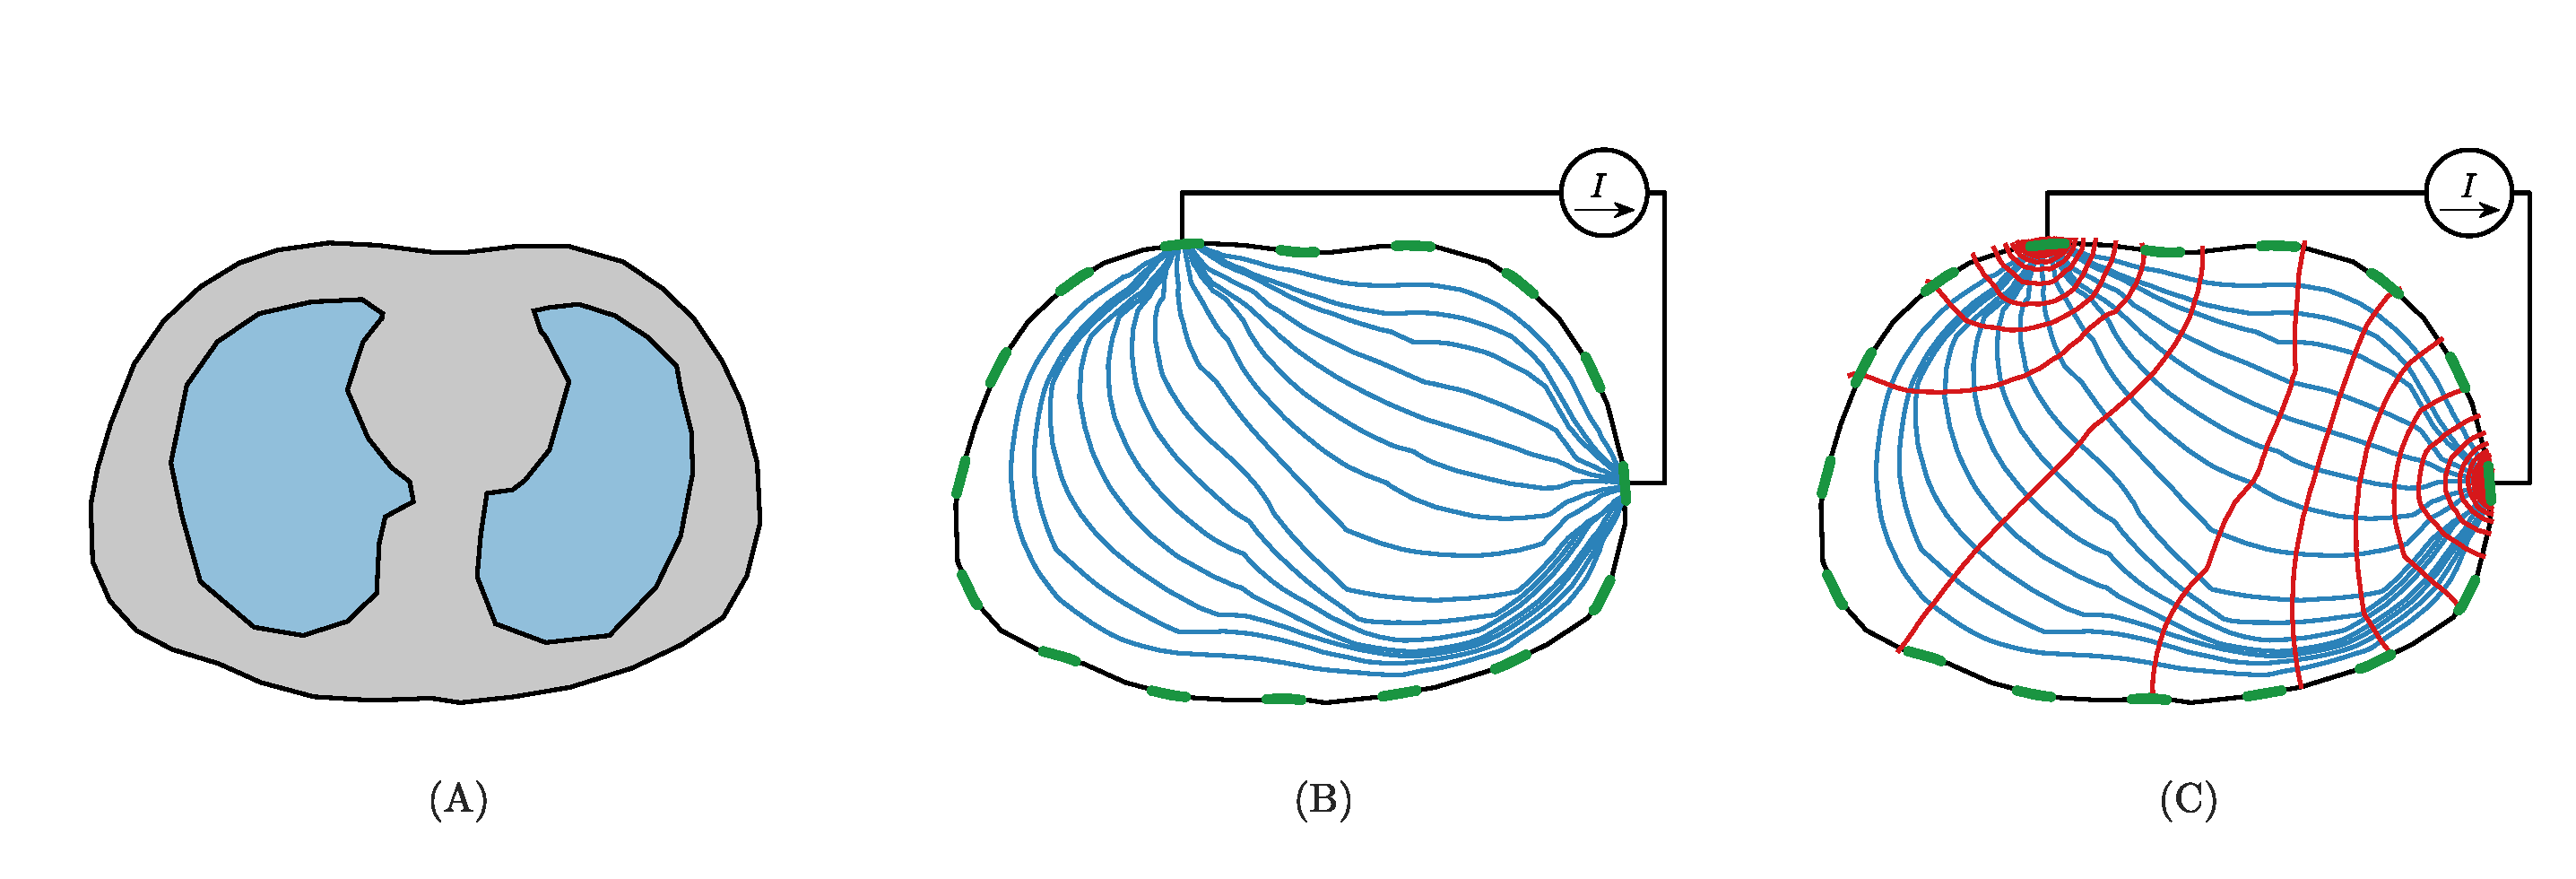
\includegraphics[width=\textwidth,trim={0 2cm 0 0},clip]{imgs/current_and_equipotential_lines.pdf}
	\end{figure}
	\vspace{2mm}
	Electrodes on the body surface are used to inject current and measure the resulting voltages. \\
	\vspace{0.5cm}
	Thoracic EIT typically images impedance changes due to the movement of fluid in the chest. \\
\end{frame}

\begin{frame}
	\frametitle{Background: Perfusion}
	What is perfusion?
\end{frame}

\begin{frame}
	\frametitle{Background: EIT Measures of Perfusion}
	How is perfusion measured? 
	Why EIT? 
	Why does it need to be improved?
\end{frame}

\begin{frame}
	\frametitle{Chapter 3: Introduction}
	There are \alert{three common techniques} to measure perfusion with EIT. 
	\begin{enumerate}
		\item Ensemble averaging
		\item Frequency filtering
		\item Bolus injection 
	\end{enumerate}
	\begin{itemize}
		\item Explore different measures of perfusion
		\item 
	\end{itemize}

\end{frame}


\begin{frame}
\frametitle{ARDS - Acute Respiratory Distress Syndrome}    
\begin{itemize}
	\item Widespread inflammation in the lungs 
	\item Reduces the lungs’ ability to exchange oxygen and carbon dioxide
	\item Can be diagnosed with chest x-ray 
	\item Treated with mechanical ventilation
\end{itemize}
\end{frame}


\begin{frame}
	\frametitle{EIT - Electrical Impedance Tomography}    
	\begin{columns}[c]
		\begin{column}{0.5\textwidth}
			\begin{figure}
				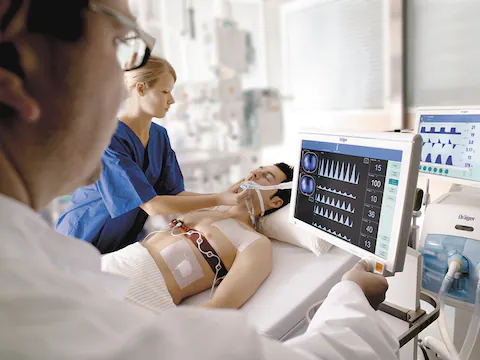
\includegraphics[width=\textwidth]{draeger_system.png}
				%\caption{Image from: drager.com}
			\end{figure}
		\end{column}
		\begin{column}{0.5\textwidth}
			\begin{itemize}
				\item used as a tool to monitor and guide mechanical ventilation  
				\item non-invasive 
				\item continuous 
				\item low-cost
				\item safe 
			\end{itemize}
		\end{column}
	\end{columns}
\end{frame}

\begin{frame}
	\frametitle{EIT - A brief overview}    
\begin{columns}[c]
	\begin{column}{0.5\textwidth}
		\begin{figure}[H]
			\centering
			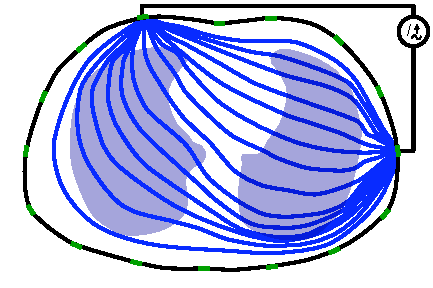
\includegraphics[width=0.9\textwidth]{current_density_injection.pdf}
		\end{figure}
	\end{column}
	\begin{column}{0.5\textwidth}
		\begin{itemize}
			\item \alert{current (blue) is injected between electrodes}
			\item voltage is measured at the body surface
			\item voltages are reconstructed into images
		\end{itemize}
	\end{column}
\end{columns}
\end{frame}

\begin{frame}
\frametitle{EIT - A brief overview}    
\begin{columns}[c]
	\begin{column}{0.5\textwidth}
		\begin{figure}[H]
			\centering
			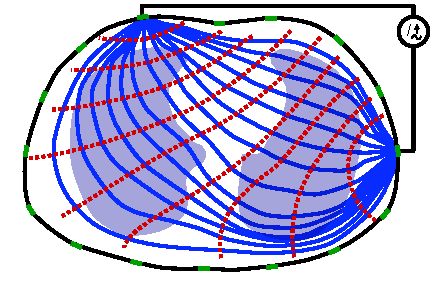
\includegraphics[width=0.9\textwidth]{current_density_voltage.pdf}
		\end{figure}
	\end{column}
	\begin{column}{0.5\textwidth}
		\begin{itemize}
			\item current (blue) is injected between electrodes
			\item \alert{voltage is measured at the body surface}
			\item voltages are reconstructed into images
		\end{itemize}
	\end{column}
\end{columns}
\end{frame}

\begin{frame}
\frametitle{EIT - A brief overview}    
\begin{columns}[c]
	\begin{column}{0.5\textwidth}
		\begin{figure}[H]
			\centering
			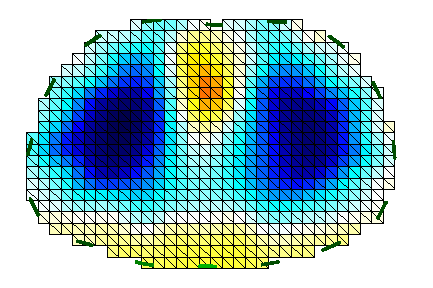
\includegraphics[width=0.9\textwidth]{current_density_image.pdf}
		\end{figure}
	\end{column}
	\begin{column}{0.5\textwidth}
		\begin{itemize}
			\item current (blue) is injected between electrodes
			\item voltage is measured at the body surface
			\item \alert{voltages are reconstructed into images}
		\end{itemize}
	\end{column}
\end{columns}
\end{frame}

\begin{frame}
	\frametitle{Finitie Element Models (FEMs) in EIT}    
	\begin{columns}[c]
		\begin{column}{0.5\textwidth}
			\begin{figure}[H]
				\centering
				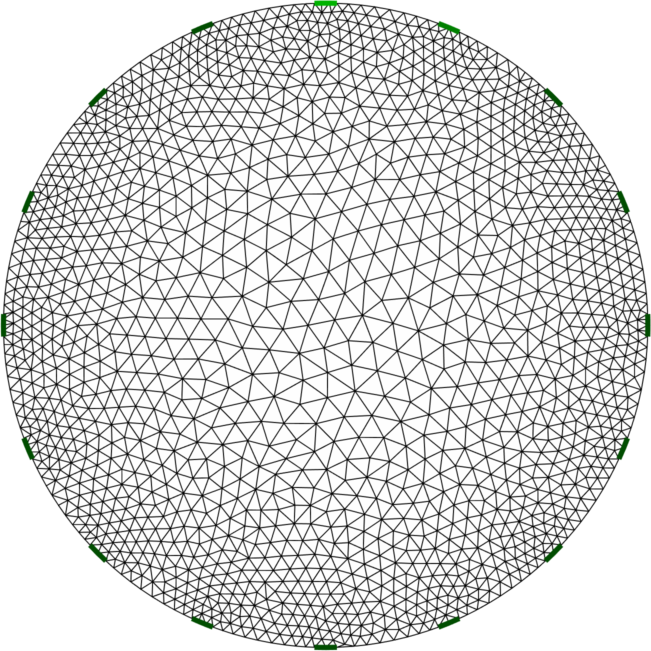
\includegraphics[width=0.9\textwidth]{basic_mesh.png}
			\end{figure}
		\end{column}
		\begin{column}{0.5\textwidth}
			\begin{itemize}
				\item \alert{finite element model is required to reconstruct voltages into images}
				\item The more accurate the FEM the better the reconstruction  
				\item More prior information regarding the body conductivity is better
			\end{itemize}
		\end{column}
	\end{columns}
\end{frame}

\begin{frame}
	\frametitle{Finitie Element Models (FEMs) in EIT}    
	\begin{columns}[c]
		\begin{column}{0.5\textwidth}
			\begin{figure}[H]
				\centering
				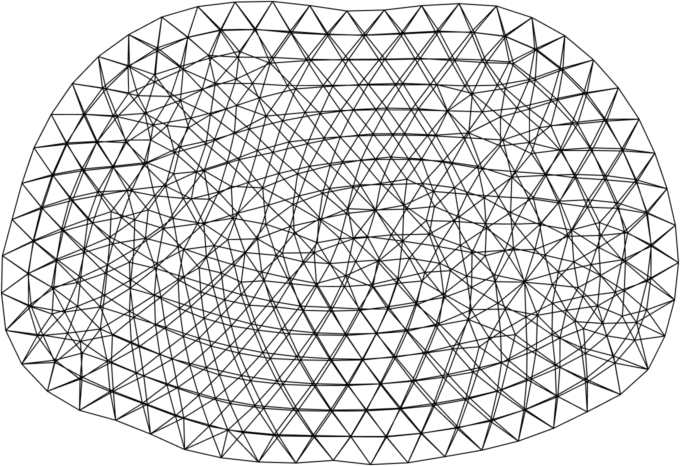
\includegraphics[width=0.9\textwidth]{human_mesh_empty.png}
			\end{figure}
		\end{column}
		\begin{column}{0.5\textwidth}
			\begin{itemize}
				\item finite element model is required to reconstruct voltages into images
				\item \alert{The more accurate the FEM the better the reconstruction} 
				\item More prior information regarding the body conductivity is better
			\end{itemize}
		\end{column}
	\end{columns}
\end{frame}

\begin{frame}
	\frametitle{Finitie Element Models (FEMs) in EIT}    
	\begin{columns}[c]
		\begin{column}{0.5\textwidth}
			\begin{figure}[H]
				\centering
				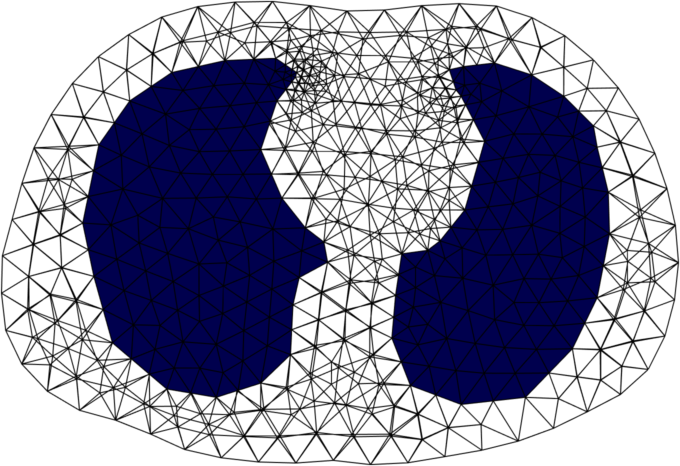
\includegraphics[width=0.9\textwidth]{human_mesh_lungs.png}
			\end{figure}
		\end{column}
		\begin{column}{0.5\textwidth}
			\begin{itemize}
				\item finite element model is required to reconstruct voltages into images
				\item The more accurate the FEM the better the reconstruction
				\item \alert{More prior information regarding the body conductivity is better}
			\end{itemize}
		\end{column}
	\end{columns}
\end{frame}

\begin{frame}
	\frametitle{Motivation}    
	\begin{itemize}
		\item Often a generic model is used for reconstructions
		\item True electrode locations and internal geometry is unknown  
		\item With ARDS patients we have information from  diagnostic CT images
		\item More prior information 
	\end{itemize}
\vspace{2em}
\alert{Can we use this to improve EIT image reconstruction and monitoring of patients?}
\end{frame}

\begin{frame}
	\frametitle{Overview}    
	\begin{enumerate}
		\item Obtain CT images
		\item Automatically identify lung regions  
		\item Present in a GUI for correction by doctors or technicians
		\item Generate a FEM based on the corrected segmentation
		\item Reconstruct EIT data
	\end{enumerate}
\end{frame}
 
 \begin{frame}
 	\frametitle{CT images}    
		\begin{figure}[H]
			\centering
			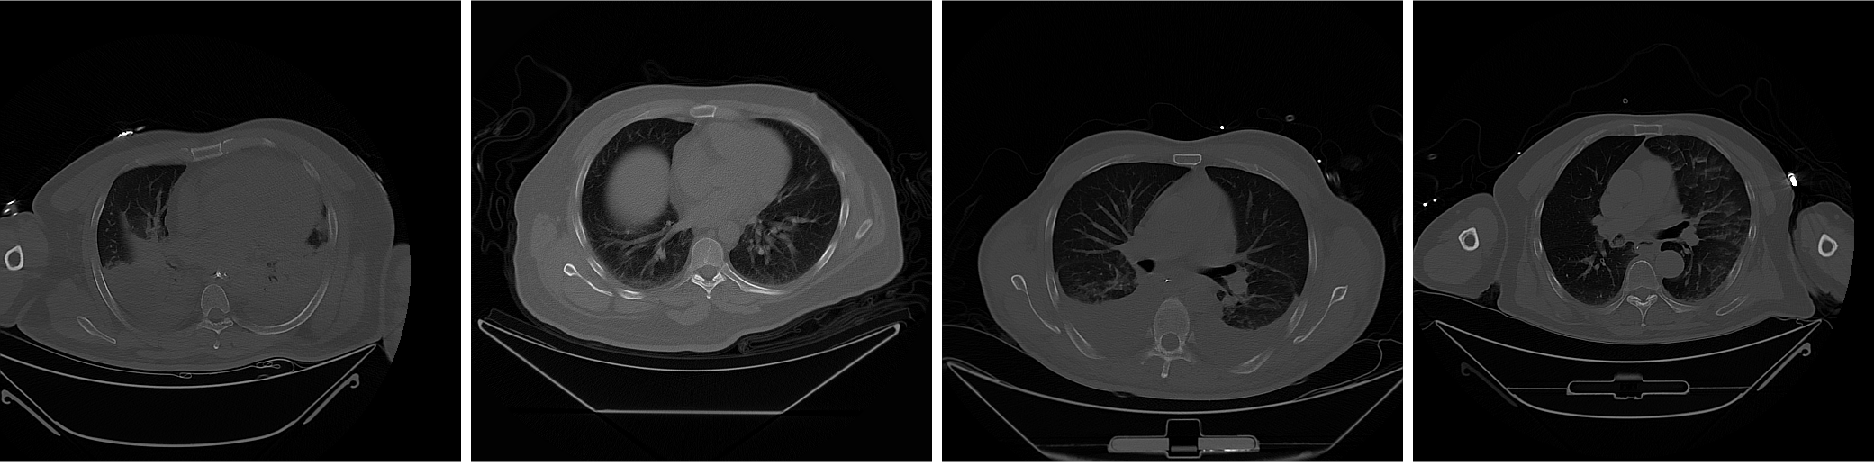
\includegraphics[width=\textwidth]{raw_ct_imgs.png}
		\end{figure}
	Example images taken from the 4th intercostal space for each subject
 \end{frame}
 
\begin{frame}
	\frametitle{Methods}    
		\begin{figure}[H]
			\centering
			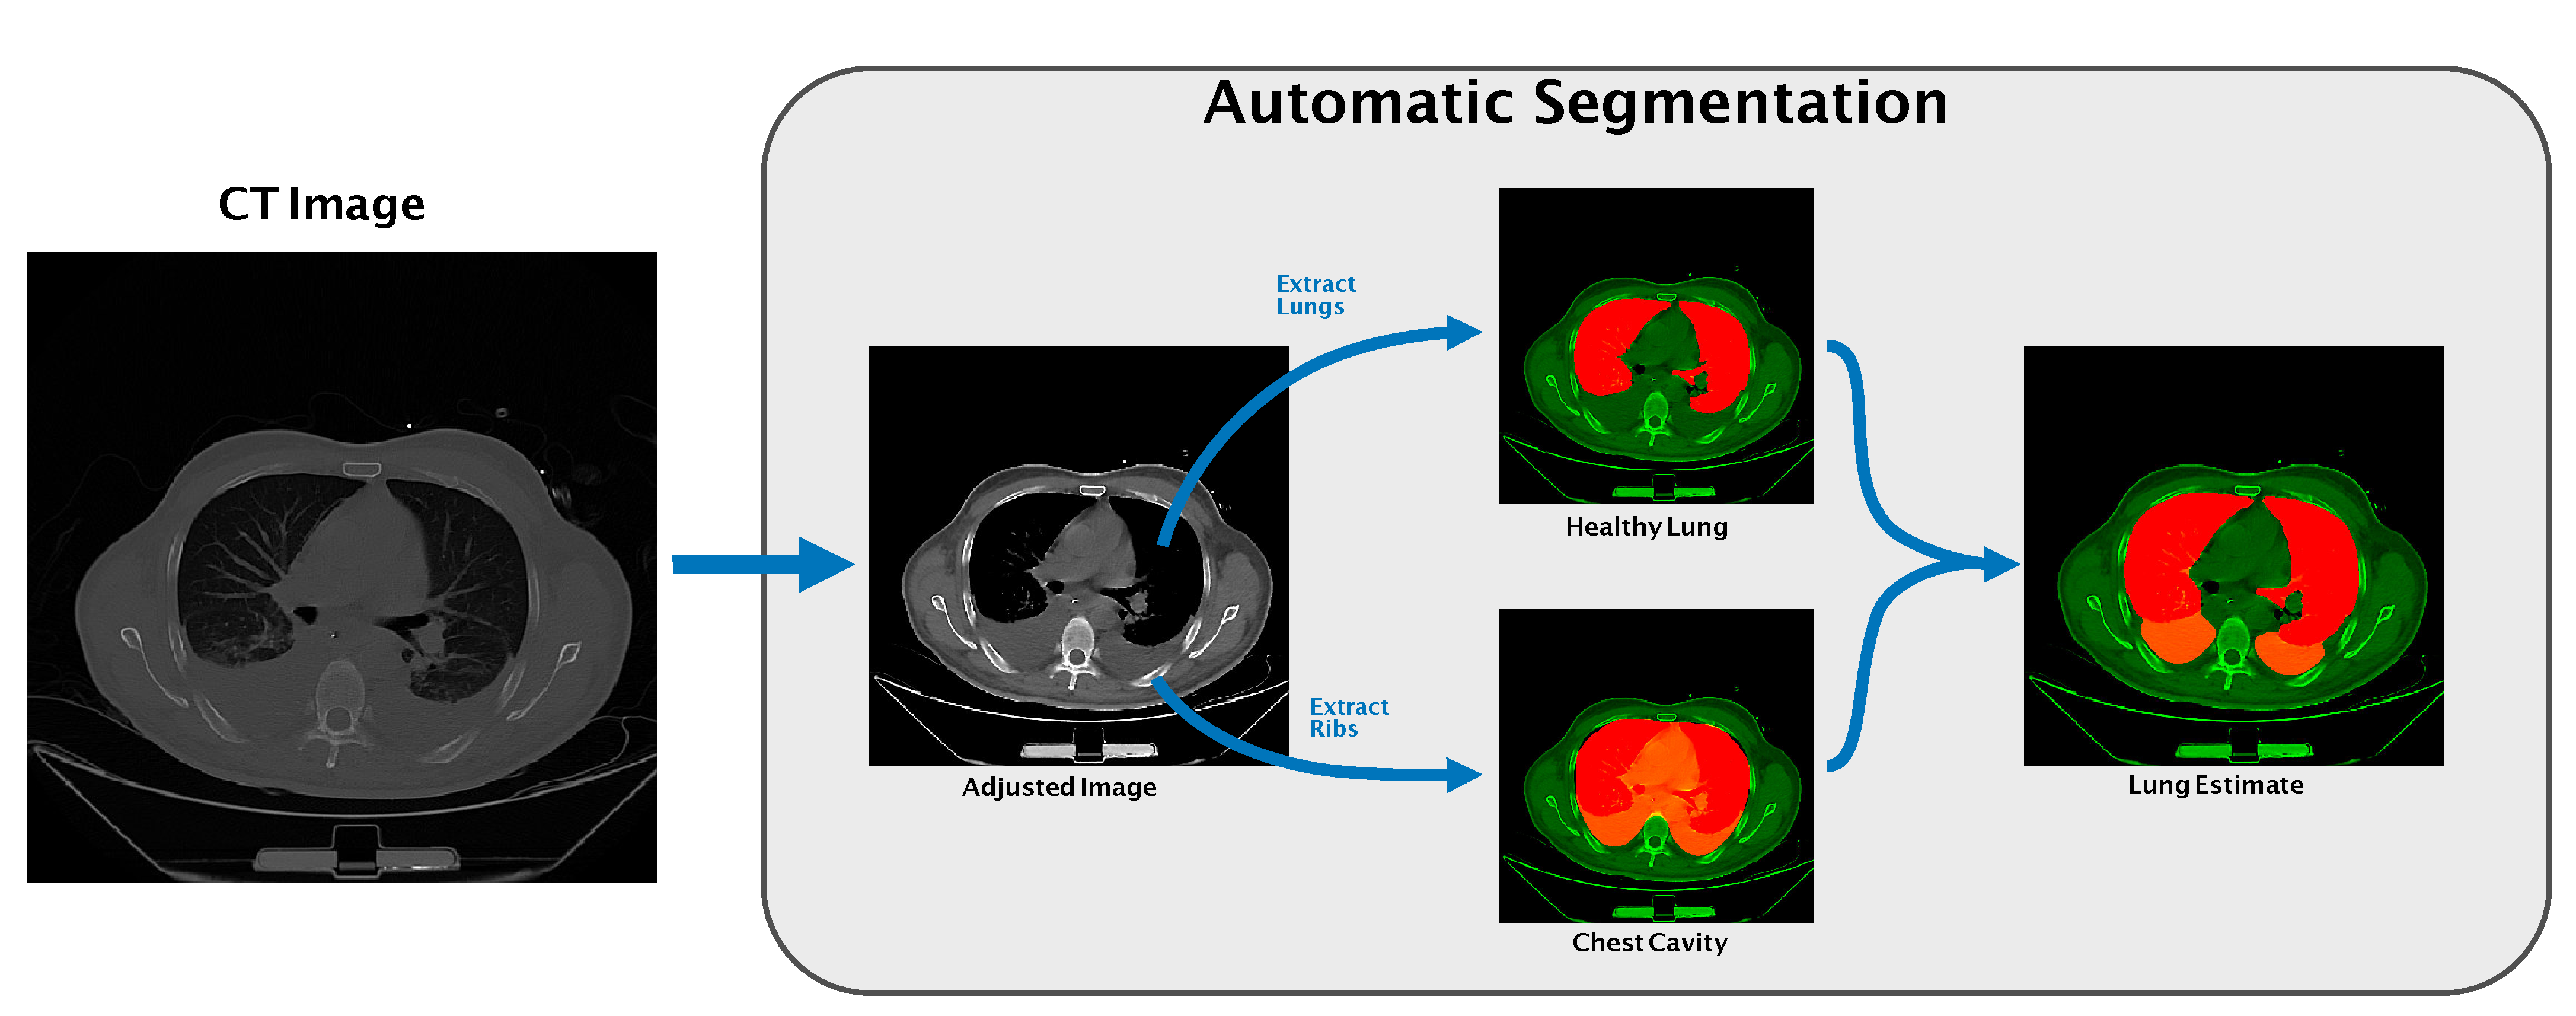
\includegraphics[width=\textwidth]{lung_segmentation_methods_a.pdf}
		\end{figure}
\end{frame}

\begin{frame}
	\frametitle{Segmentation Results}    
	\begin{figure}[H]
		\centering
		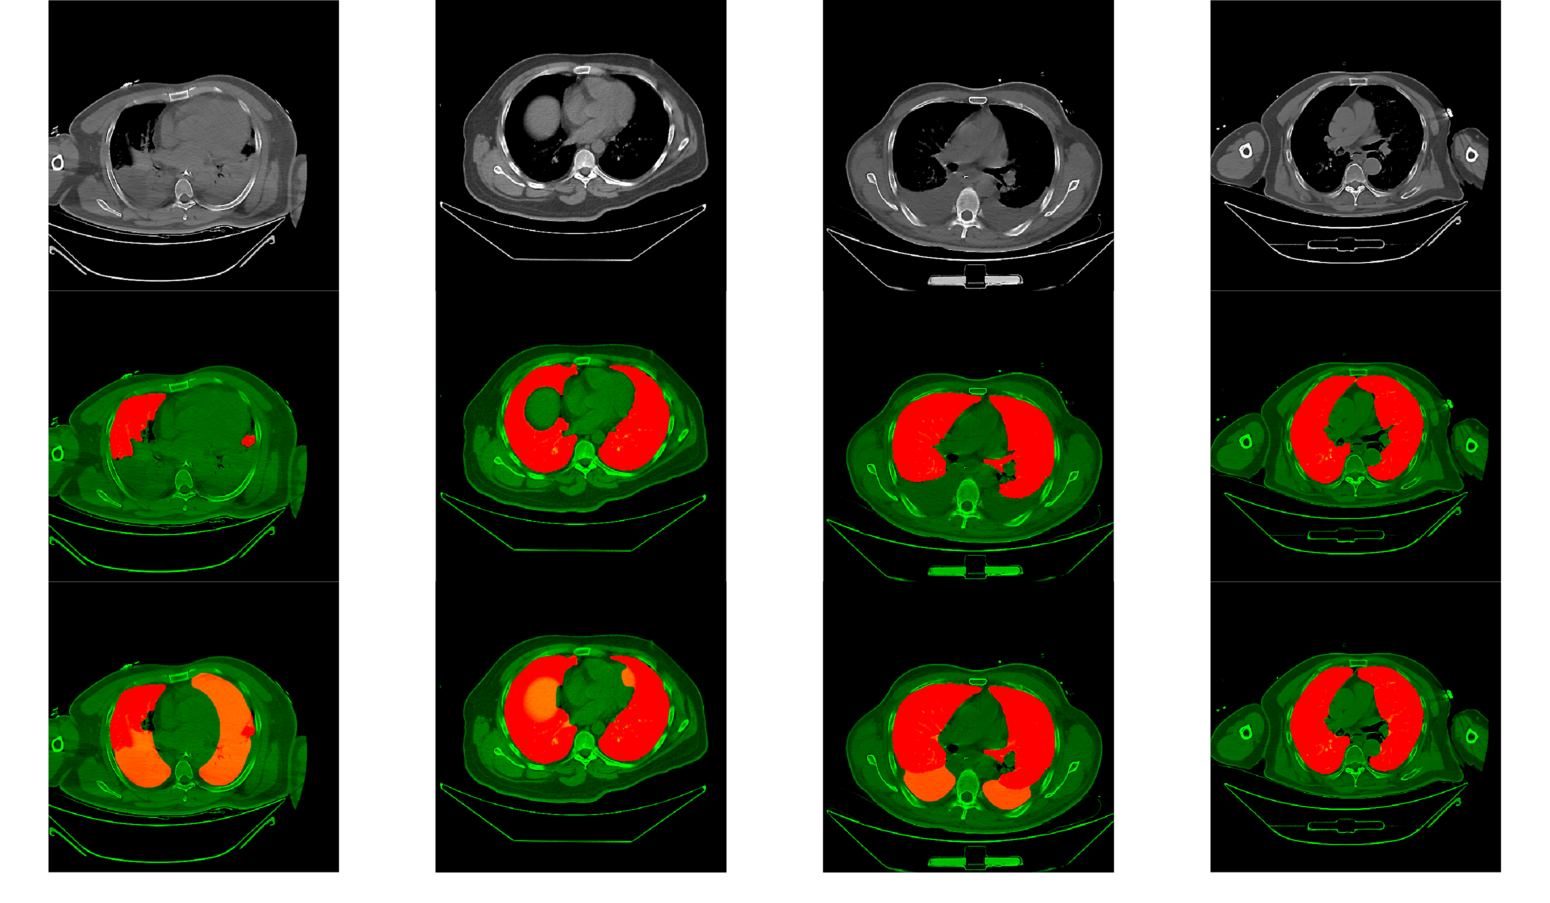
\includegraphics[width=\textwidth]{segment_results.png}
	\end{figure}
\end{frame}

\begin{frame}
	\frametitle{Methods}    
	\begin{figure}[H]
		\centering
		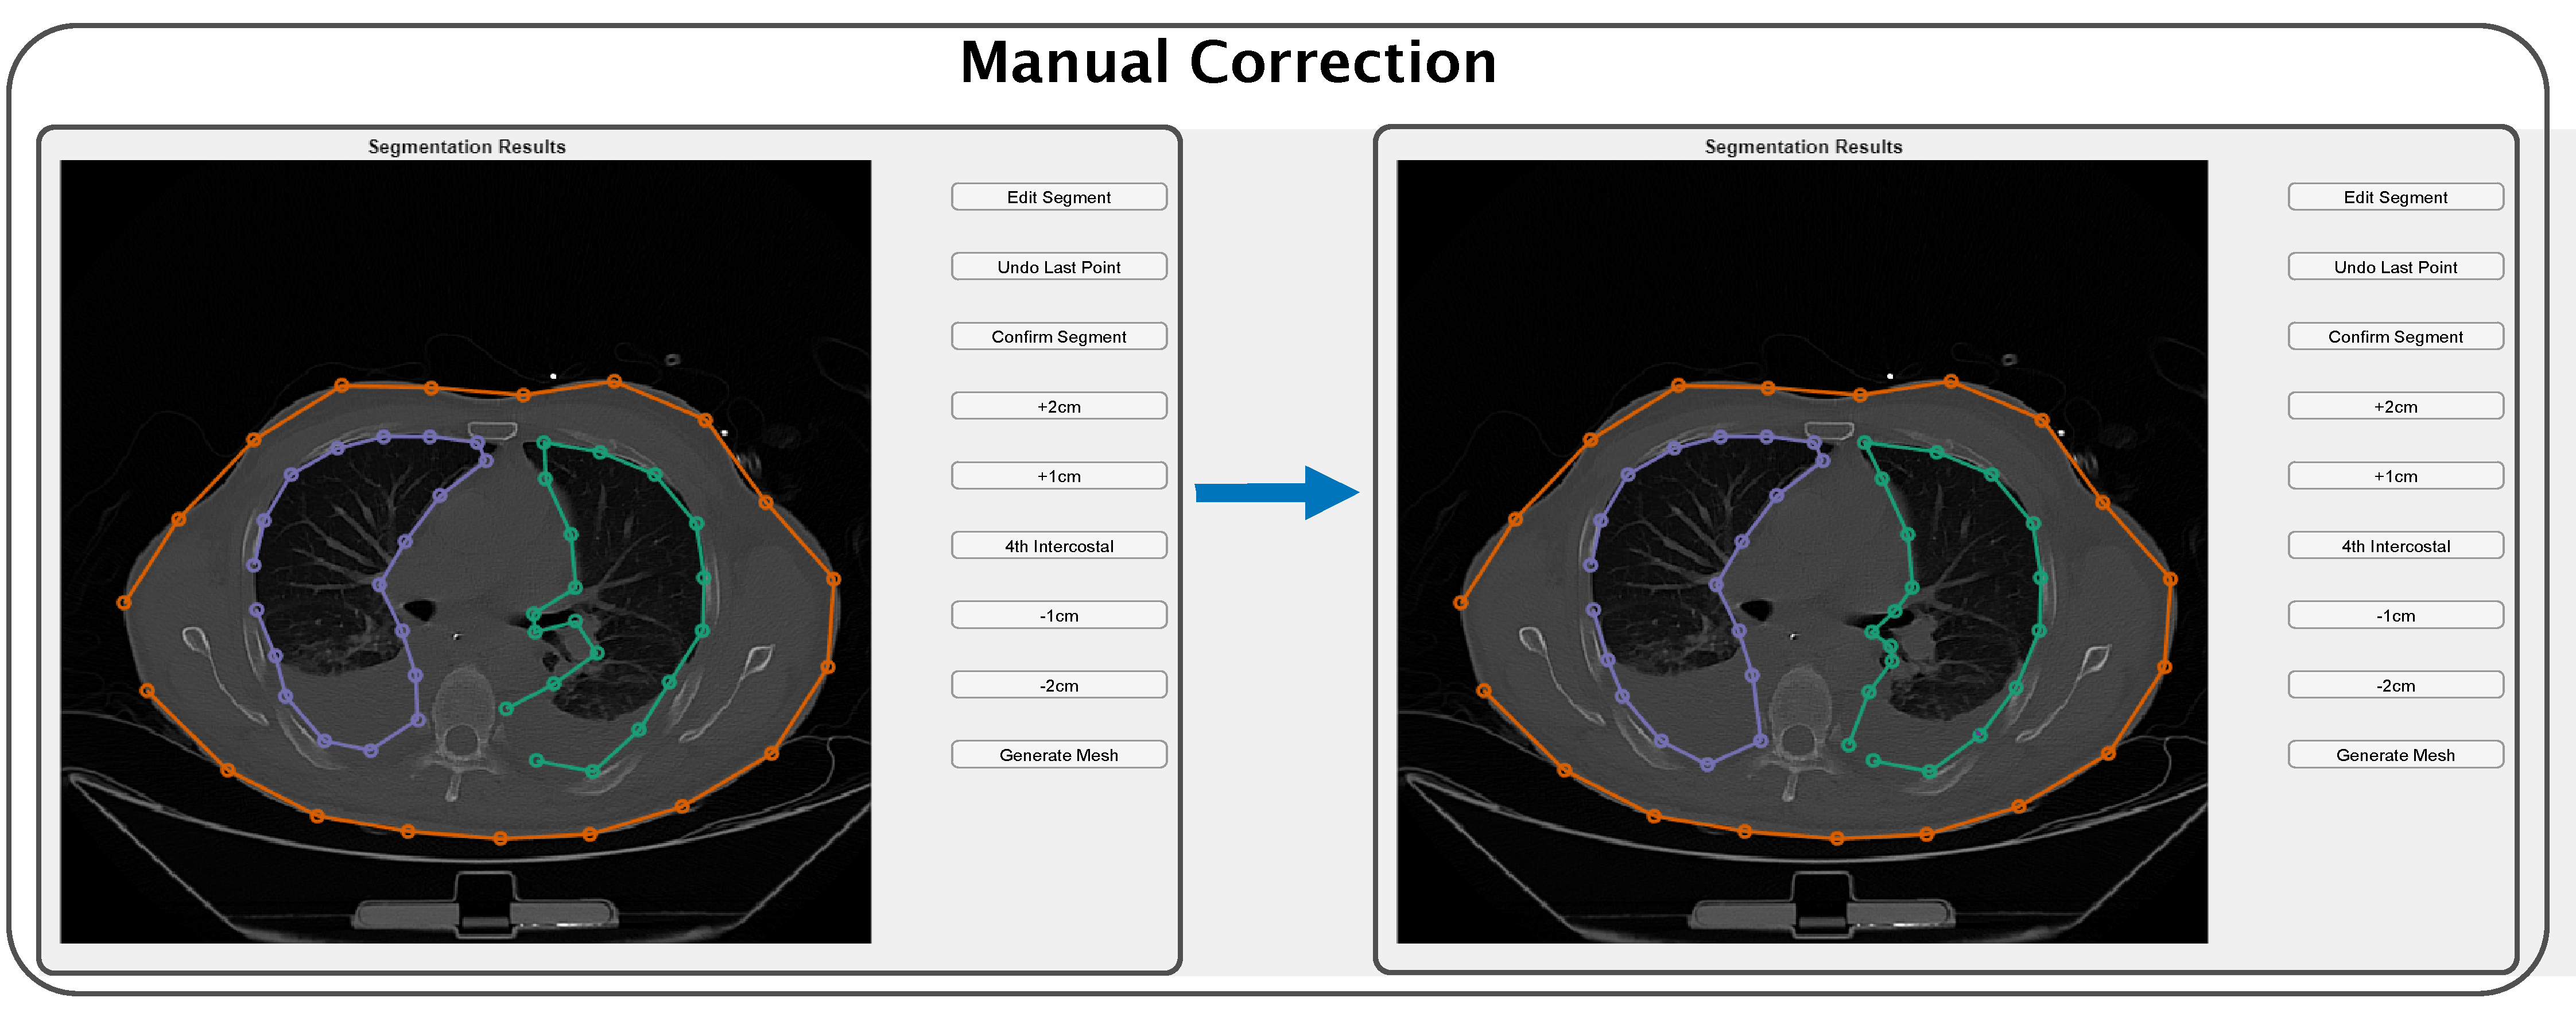
\includegraphics[width=\textwidth]{lung_segmentation_methods_b.pdf}
	\end{figure}
\end{frame}

\begin{frame}
	\frametitle{Methods}    
	\begin{figure}[H]
		\centering
		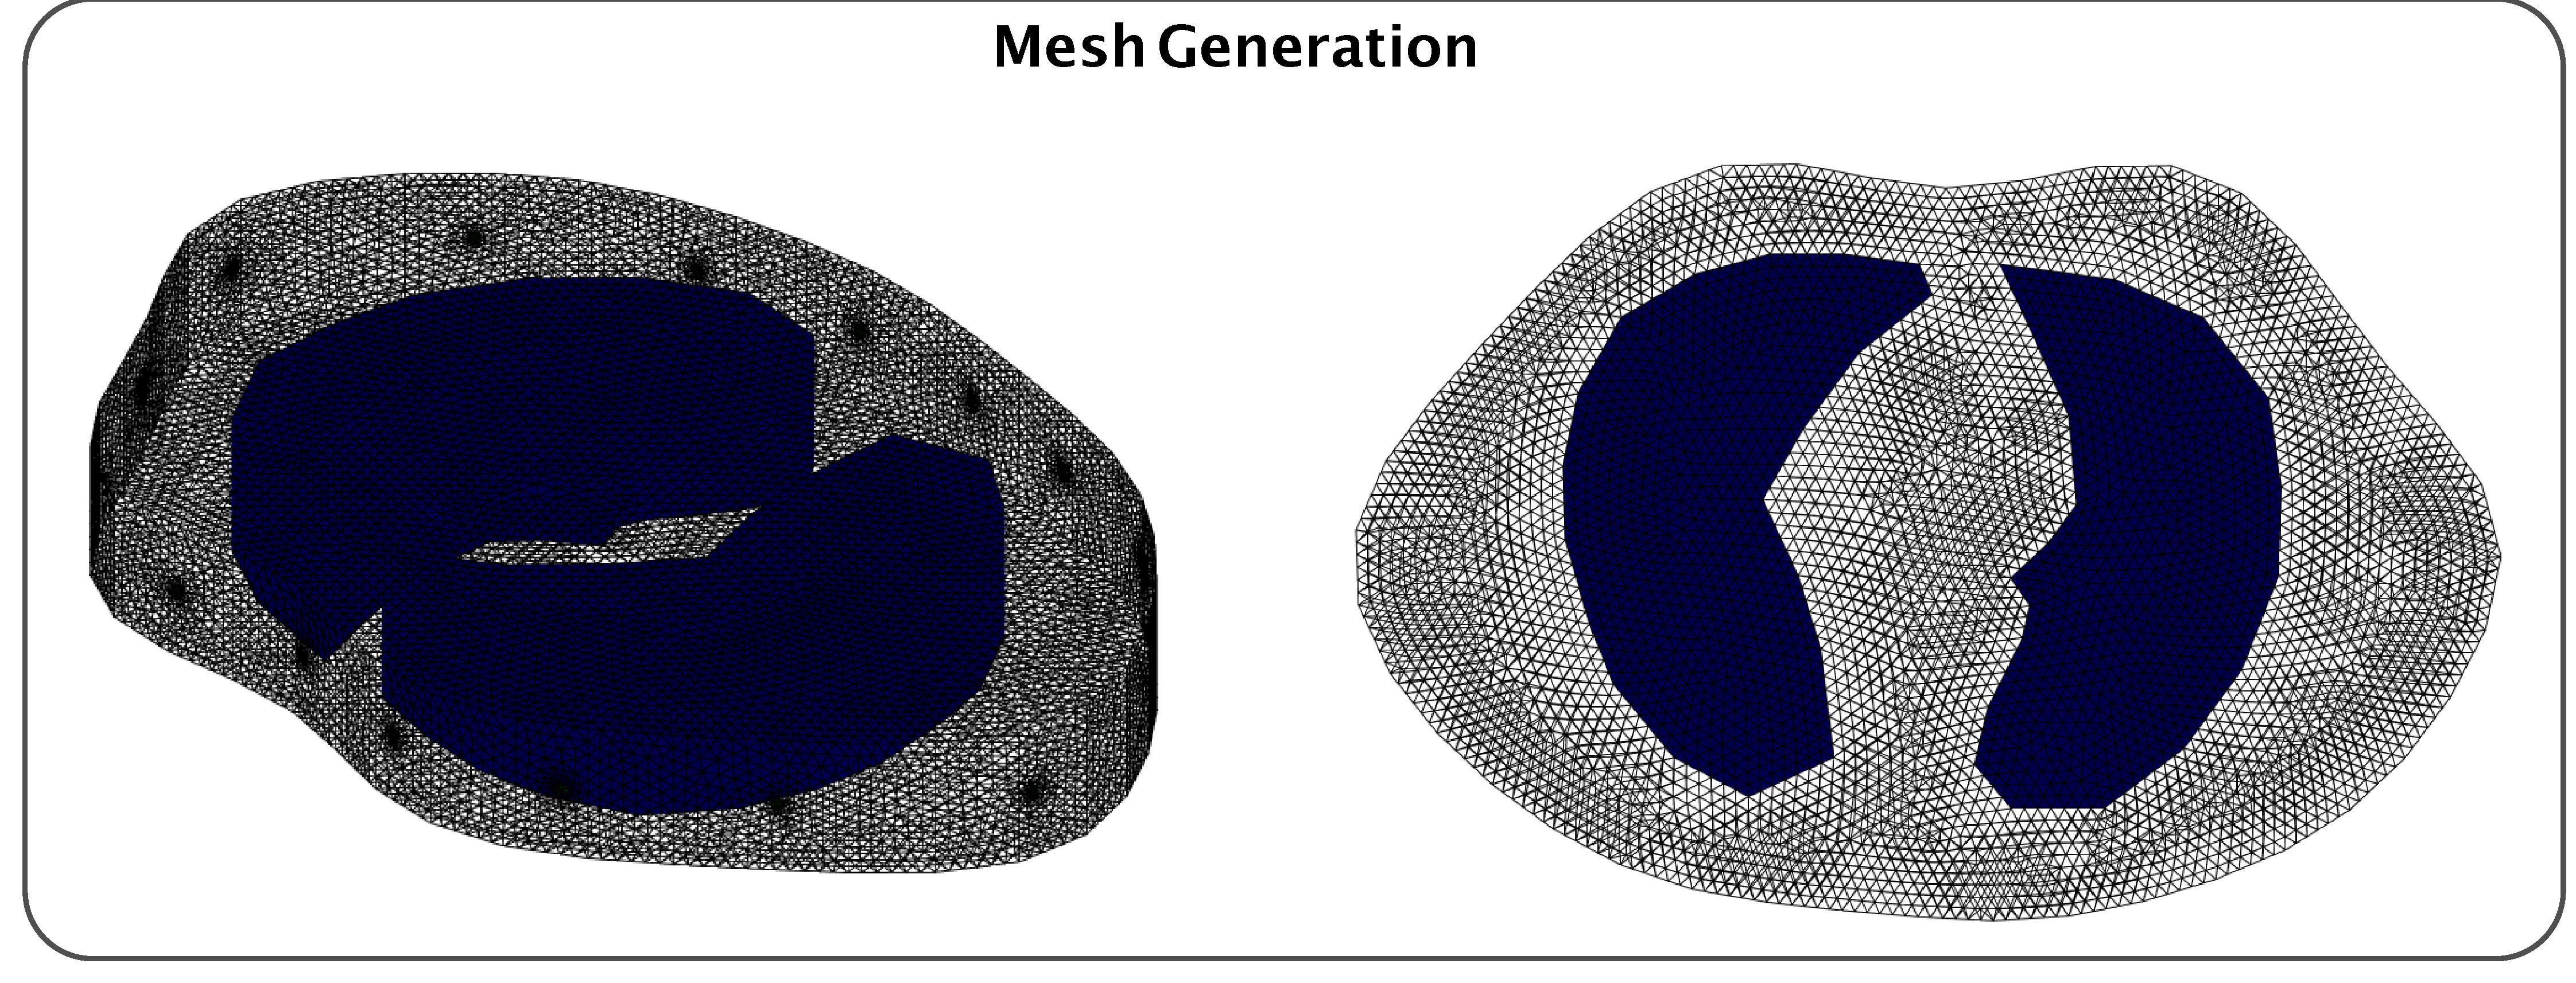
\includegraphics[width=\textwidth]{lung_segmentation_methods_c.pdf}
	\end{figure}
\end{frame}

\begin{frame}
	\frametitle{Preliminary Results}   
	\begin{columns}[c]
		\begin{column}{0.5\textwidth}
		\begin{figure}[H]
			\centering
			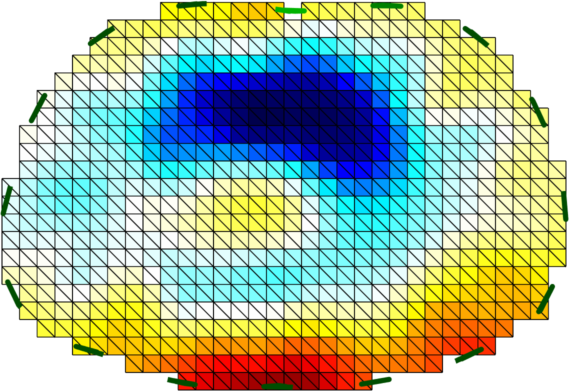
\includegraphics[width=\textwidth]{generic_fem.png}
		\end{figure}
		\end{column}
		\begin{column}{0.5\textwidth}
			\begin{figure}[H]
				\centering
				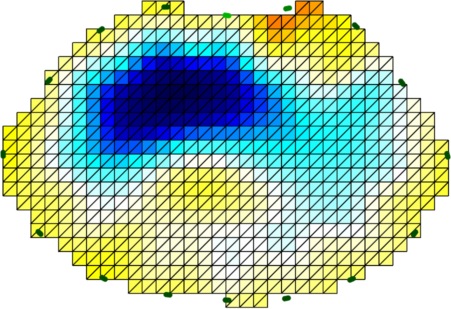
\includegraphics[width=\textwidth]{new_fem.png}
			\end{figure}
		\end{column}
	\end{columns} 
\vspace{1em}
An average breath imaged for two FEMs
	
\end{frame}

\begin{frame}
\frametitle{Current Work}    
\begin{columns}[c]
\begin{column}{0.5\textwidth}
\alert{Improvement}
\begin{itemize}
\item Apply the segmentation to larger numbers of patients
\item Create a more user friendly editing pgoram to accelerate segmentation and meshing
\item Create a database of meshes that can be applied to additional subjects
\end{itemize}
\end{column}
\begin{column}{0.5\textwidth}
\alert{Validate the use of custom meshes for ARDS monitoring} \\
\vspace{1em}
Do patient specific meshes:
\begin{itemize}
\item improve on generic meshes for ARDS monitoring?
\item give increased accuracy in measures of lung collapse and fluid movement?
\item Improve detection of collapse and overdistention 
\end{itemize}
\end{column}
\end{columns}
\end{frame}


\begin{frame}
  \titlepage
\end{frame}

%%%%%%%%%%%%%%%%%%%%%%%%%%%%%%%%%%%%%%%%%%%%%%%%%%%%%%%%%%%%%%%
\end{document}
